\chapter{Quench Recognition Problem (QRP)}
\label{chp:qrp}
This chapter is dedicated to how we handled the first of the two problems that we introduced in the
perevious chapter, since $\qlp$ is an extension of $\qrp$ we began with the analysis of the easier
problem, all of the conclusions that we reach in this chapter, as far as the interaction between the
various harmonics is concerned, can be extended to the $\qlp$ problem as well.

In this chapter we will:
\begin{itemize}
	\item Give a rapid overview of the problem,
	\item Talk about the models used and the results obtained for each model,
	\item Select the 'best' model among the possibilities and then we will back our decision.
\end{itemize}

\section{Problem description}
As was introduced in the previous chapter we were given by Samuele Mariotto a dataset containing
four tables of $279$ samples each, divided between 'quench' and 'non-quench' events, the distribution is not exactly
balanced: $192$ quench events and $87$ non-quench events. The imbalance is not
extreme, therefore we kept it in mind but without worrying about it too much.

\section{Data preprocessing}
Before working on the actual models we analyzed the data to determine how correlated were the
harmonics for each table, secondly we analyzed the amount of information that each harmonic carried
by checking their box plot, the larger the amount of variables covered by the harmonic, the more
information the harmonic carried. Lastly we computed the correlation between each harmonic and the
label (quench or non quench) associated to the table.

The results are reported in the following sections, one for each table.

\subsubsection{An table}
\Cref{img:an-corr} shows the correlation of the various harmonics with each other. Independently
of the sign of the cross-correlation measurement, the matrix has $5$ different diagonals (other than
the main diagonal) that contain repeated information, e.g., harmonic number $1$ provides the same
information as harmonic number $3, 5, 7, \ldots$.
\begin{figure}
	\centering
	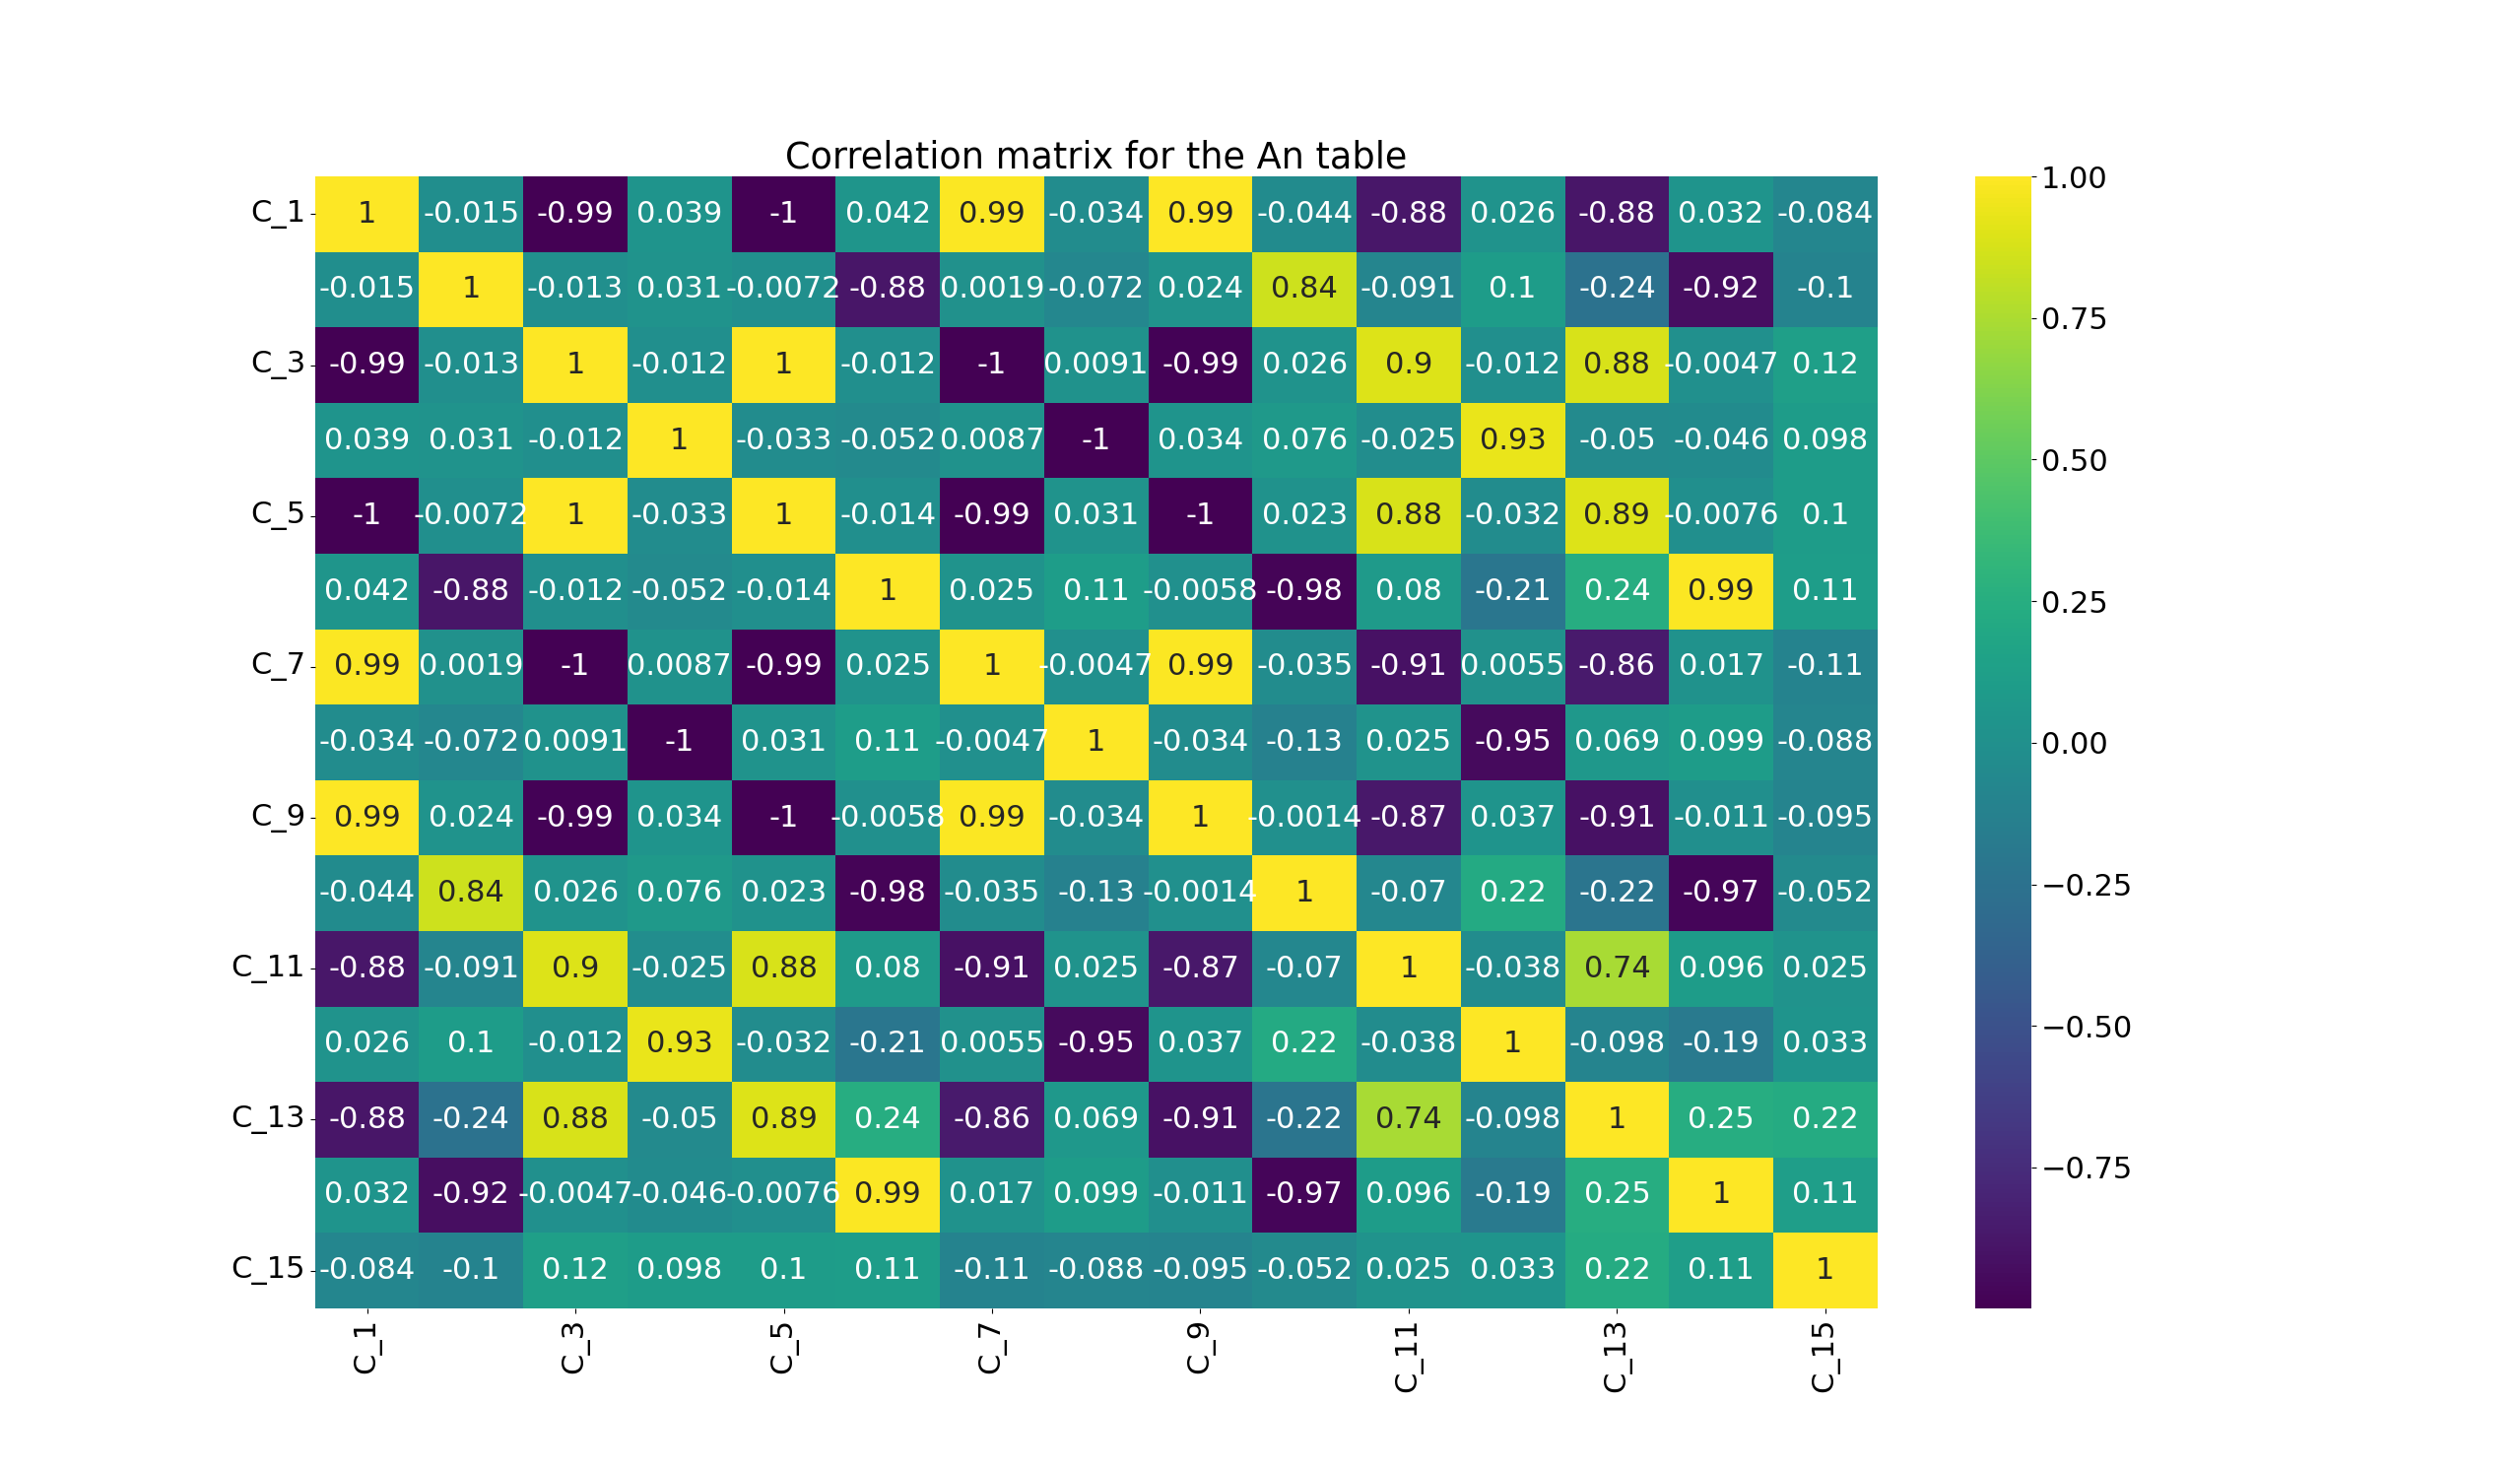
\includegraphics[scale=.25]{img/An_corr_matrix.png}
	\caption{The cross-correlation of the An harmonics} \label{fig:an-corr}
\end{figure}
Other than us noticing that the situation is definitely complex and doing feature extraction on this
matrix might be trickier than we would have otherwise assumed, we also noticed that Harmonic number
$2$ is strongly correlated with its odd multiples: $6, 10, 14$; which was expected behavior.

By looking at \Cref{fig:an-corr} we can gather the following information:
\begin{itemize}
	\item All the odd harmonics are strongly correlated with each other (with the sole exception
	      of harmonic $15$),
	\item Harmonic number $2$ is strongly correlated with its odd multiples,
	\item Harmonic number $4$ is strongly correlated with all its multiples,
	\item Harmonic number $15$ is the only one that is not correlated to any of the other
	      harmonics.
\end{itemize}

Keeping the information above in mind we can check \Cref{fig:an-lcorr} to understand which of the
harmonics best explain the expected results, and come up with different harmonic combinations that
should be performing at a high level.

\begin{figure}
	\centering
	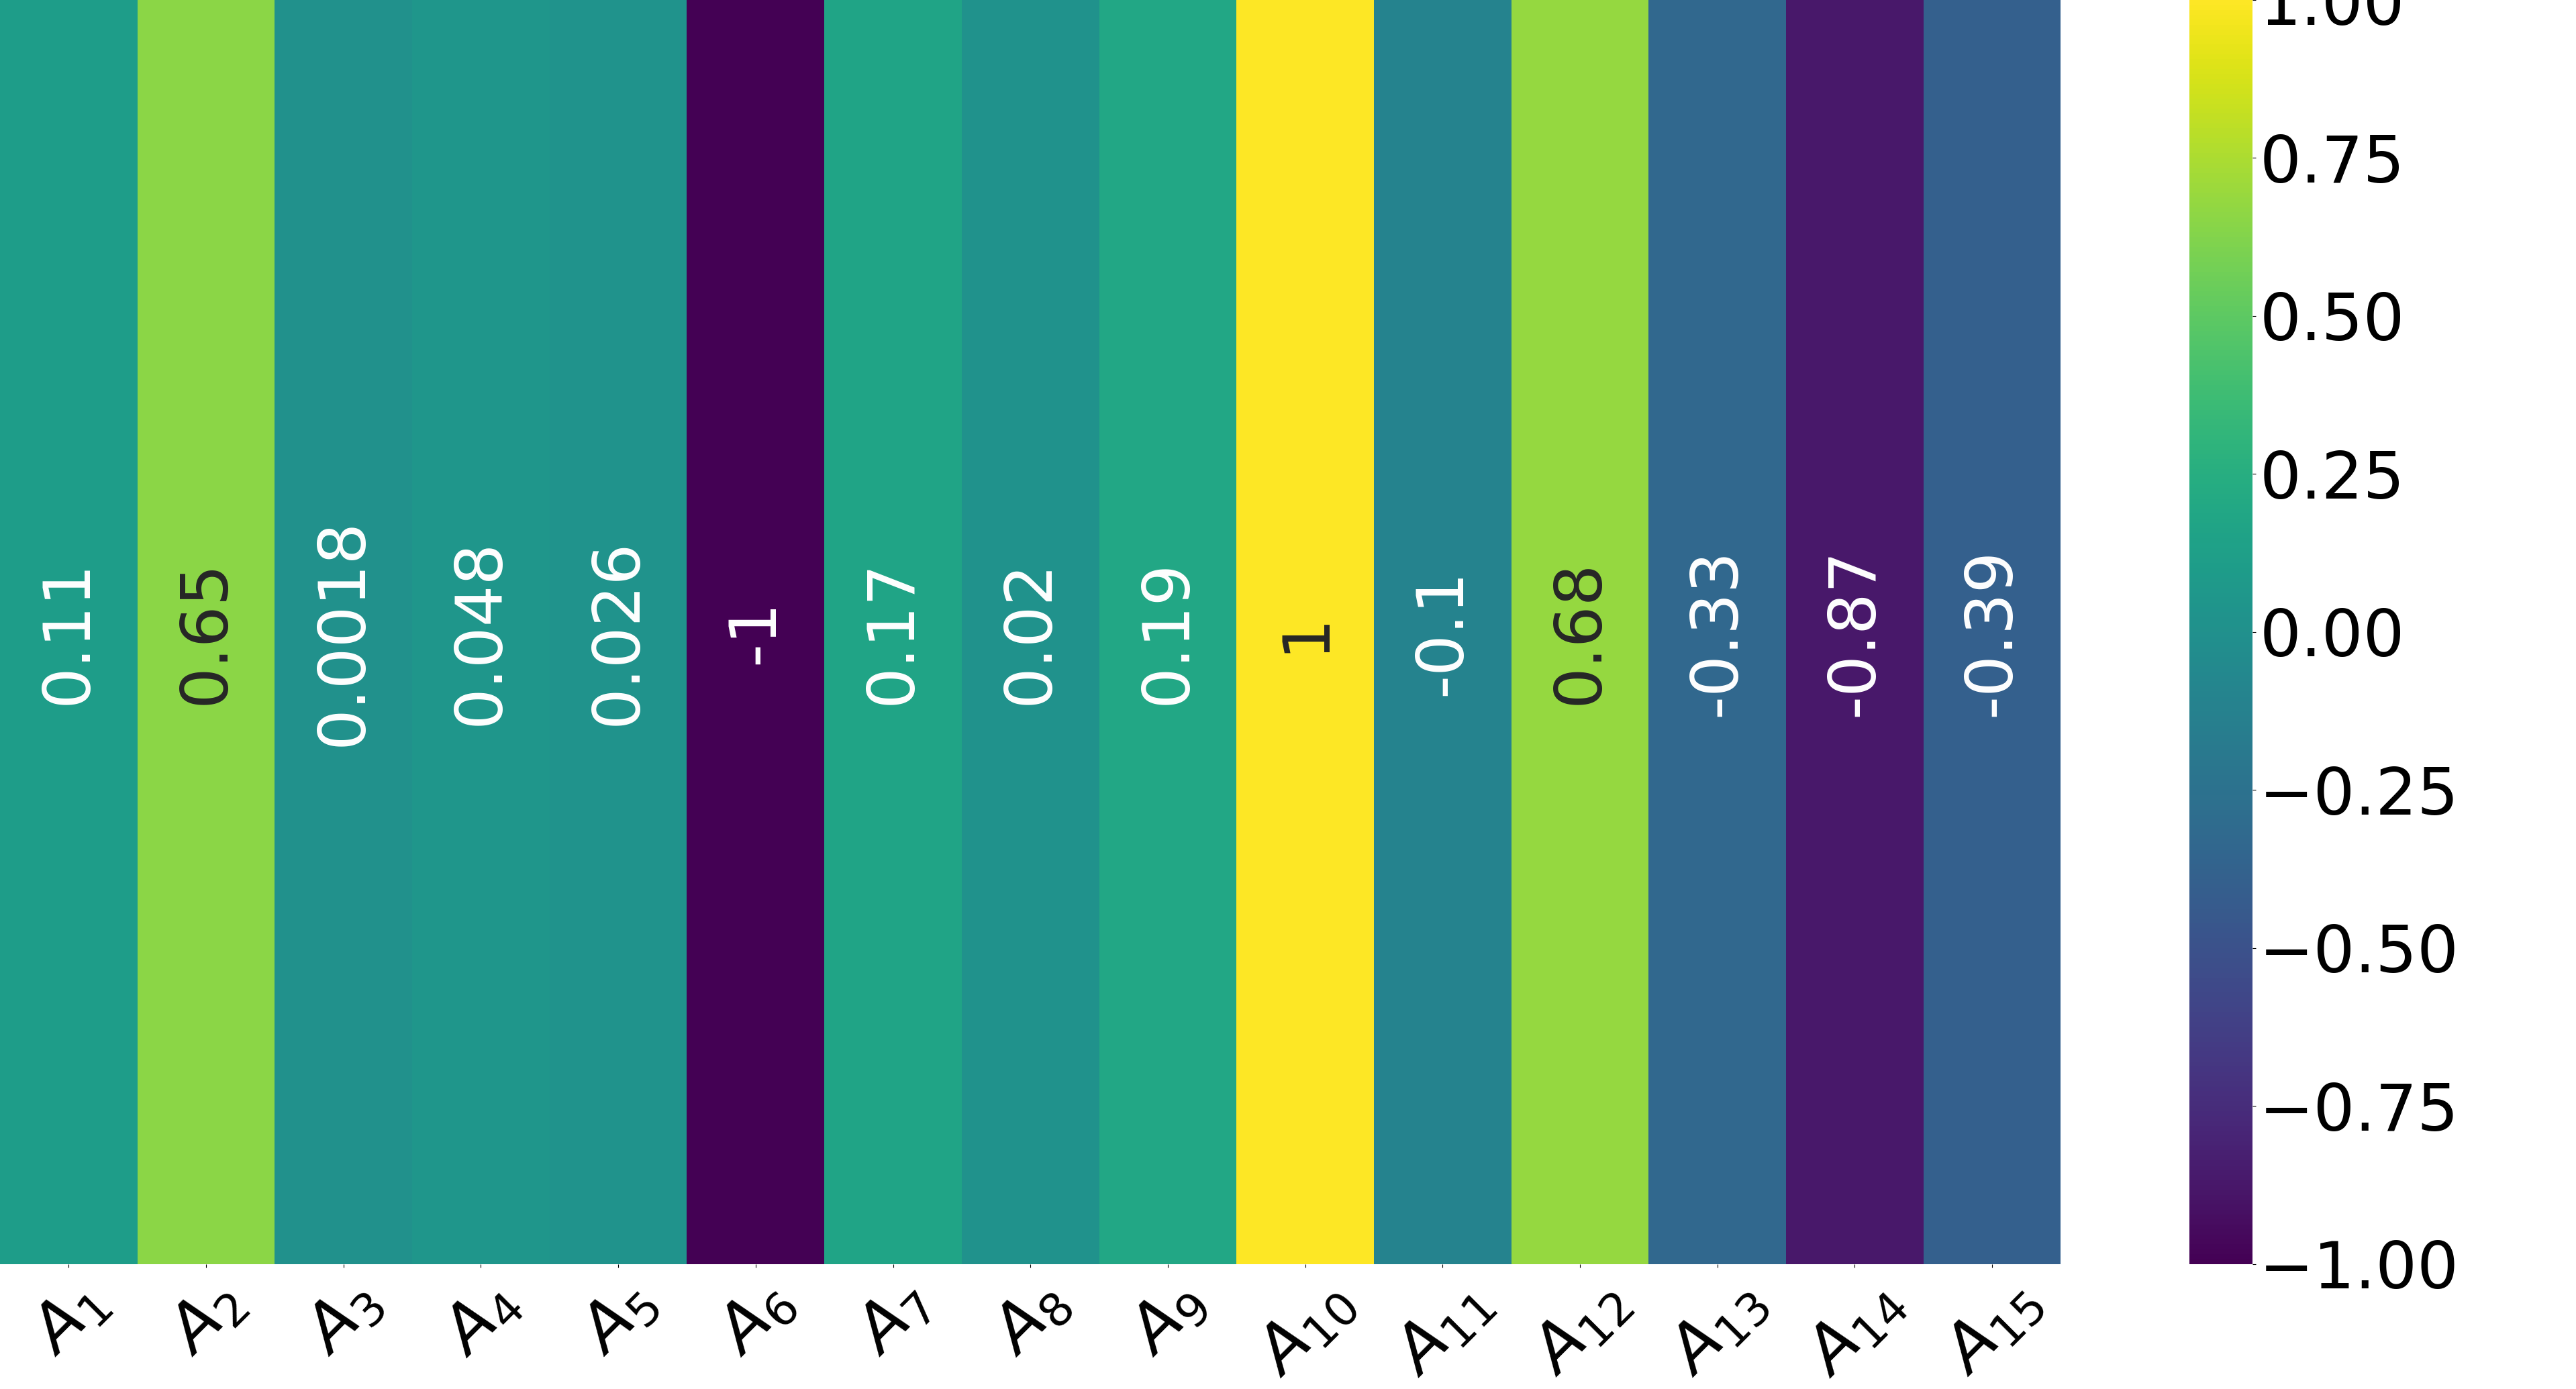
\includegraphics[scale=.25]{img/An_label_corr.png}
	\caption{Label correlation for the An table} \label{fig:an-lcorr}
\end{figure}

Once again, considering \Cref{fig:an-lcorr} we will be picking the harmonics with the highest label
correlation, which is identified by a higher color intensity. The result
is that harmonics number: $2, 6, 10, 11, 12, 13, 14, 15$; can explain the results very well, this
result is interesting on two sides:
\begin{enumerate}
	\item The $2^{nd}$ harmonic, as well as its odd multiples, can explain the results well, which
	      is what we expect from the theory.
	\item High order harmonics are able to explain the results better than other harmonics,
	      which is not what we would expect, since in the original analysis the value for the
	      labels was computed using primarily lower order harmonics.
\end{enumerate}
Based on all the information obtained up to this point we can conjecture that some of the best
datasets will probably contain the second harmonic, or one of its high order odd multiples, will
likely contain harmonic number $15$, as well as some other high order harmonic that doesn't collide
with anything that has been taken previously (i.e.: harmonics number $11$ or $13$). As we will see
in the following one of the best datasets that we built on this table was based on harmonics $2, 12,
	15$.

Lastly, we can check the distribution of the samples in bidimensional space, since the data have
$15$ dimensions to be able to plot them we use a dimensionality reduction technique, namely
$\textsc{pca}$ (Principal Component Analysis).
\begin{figure}
	\centering
	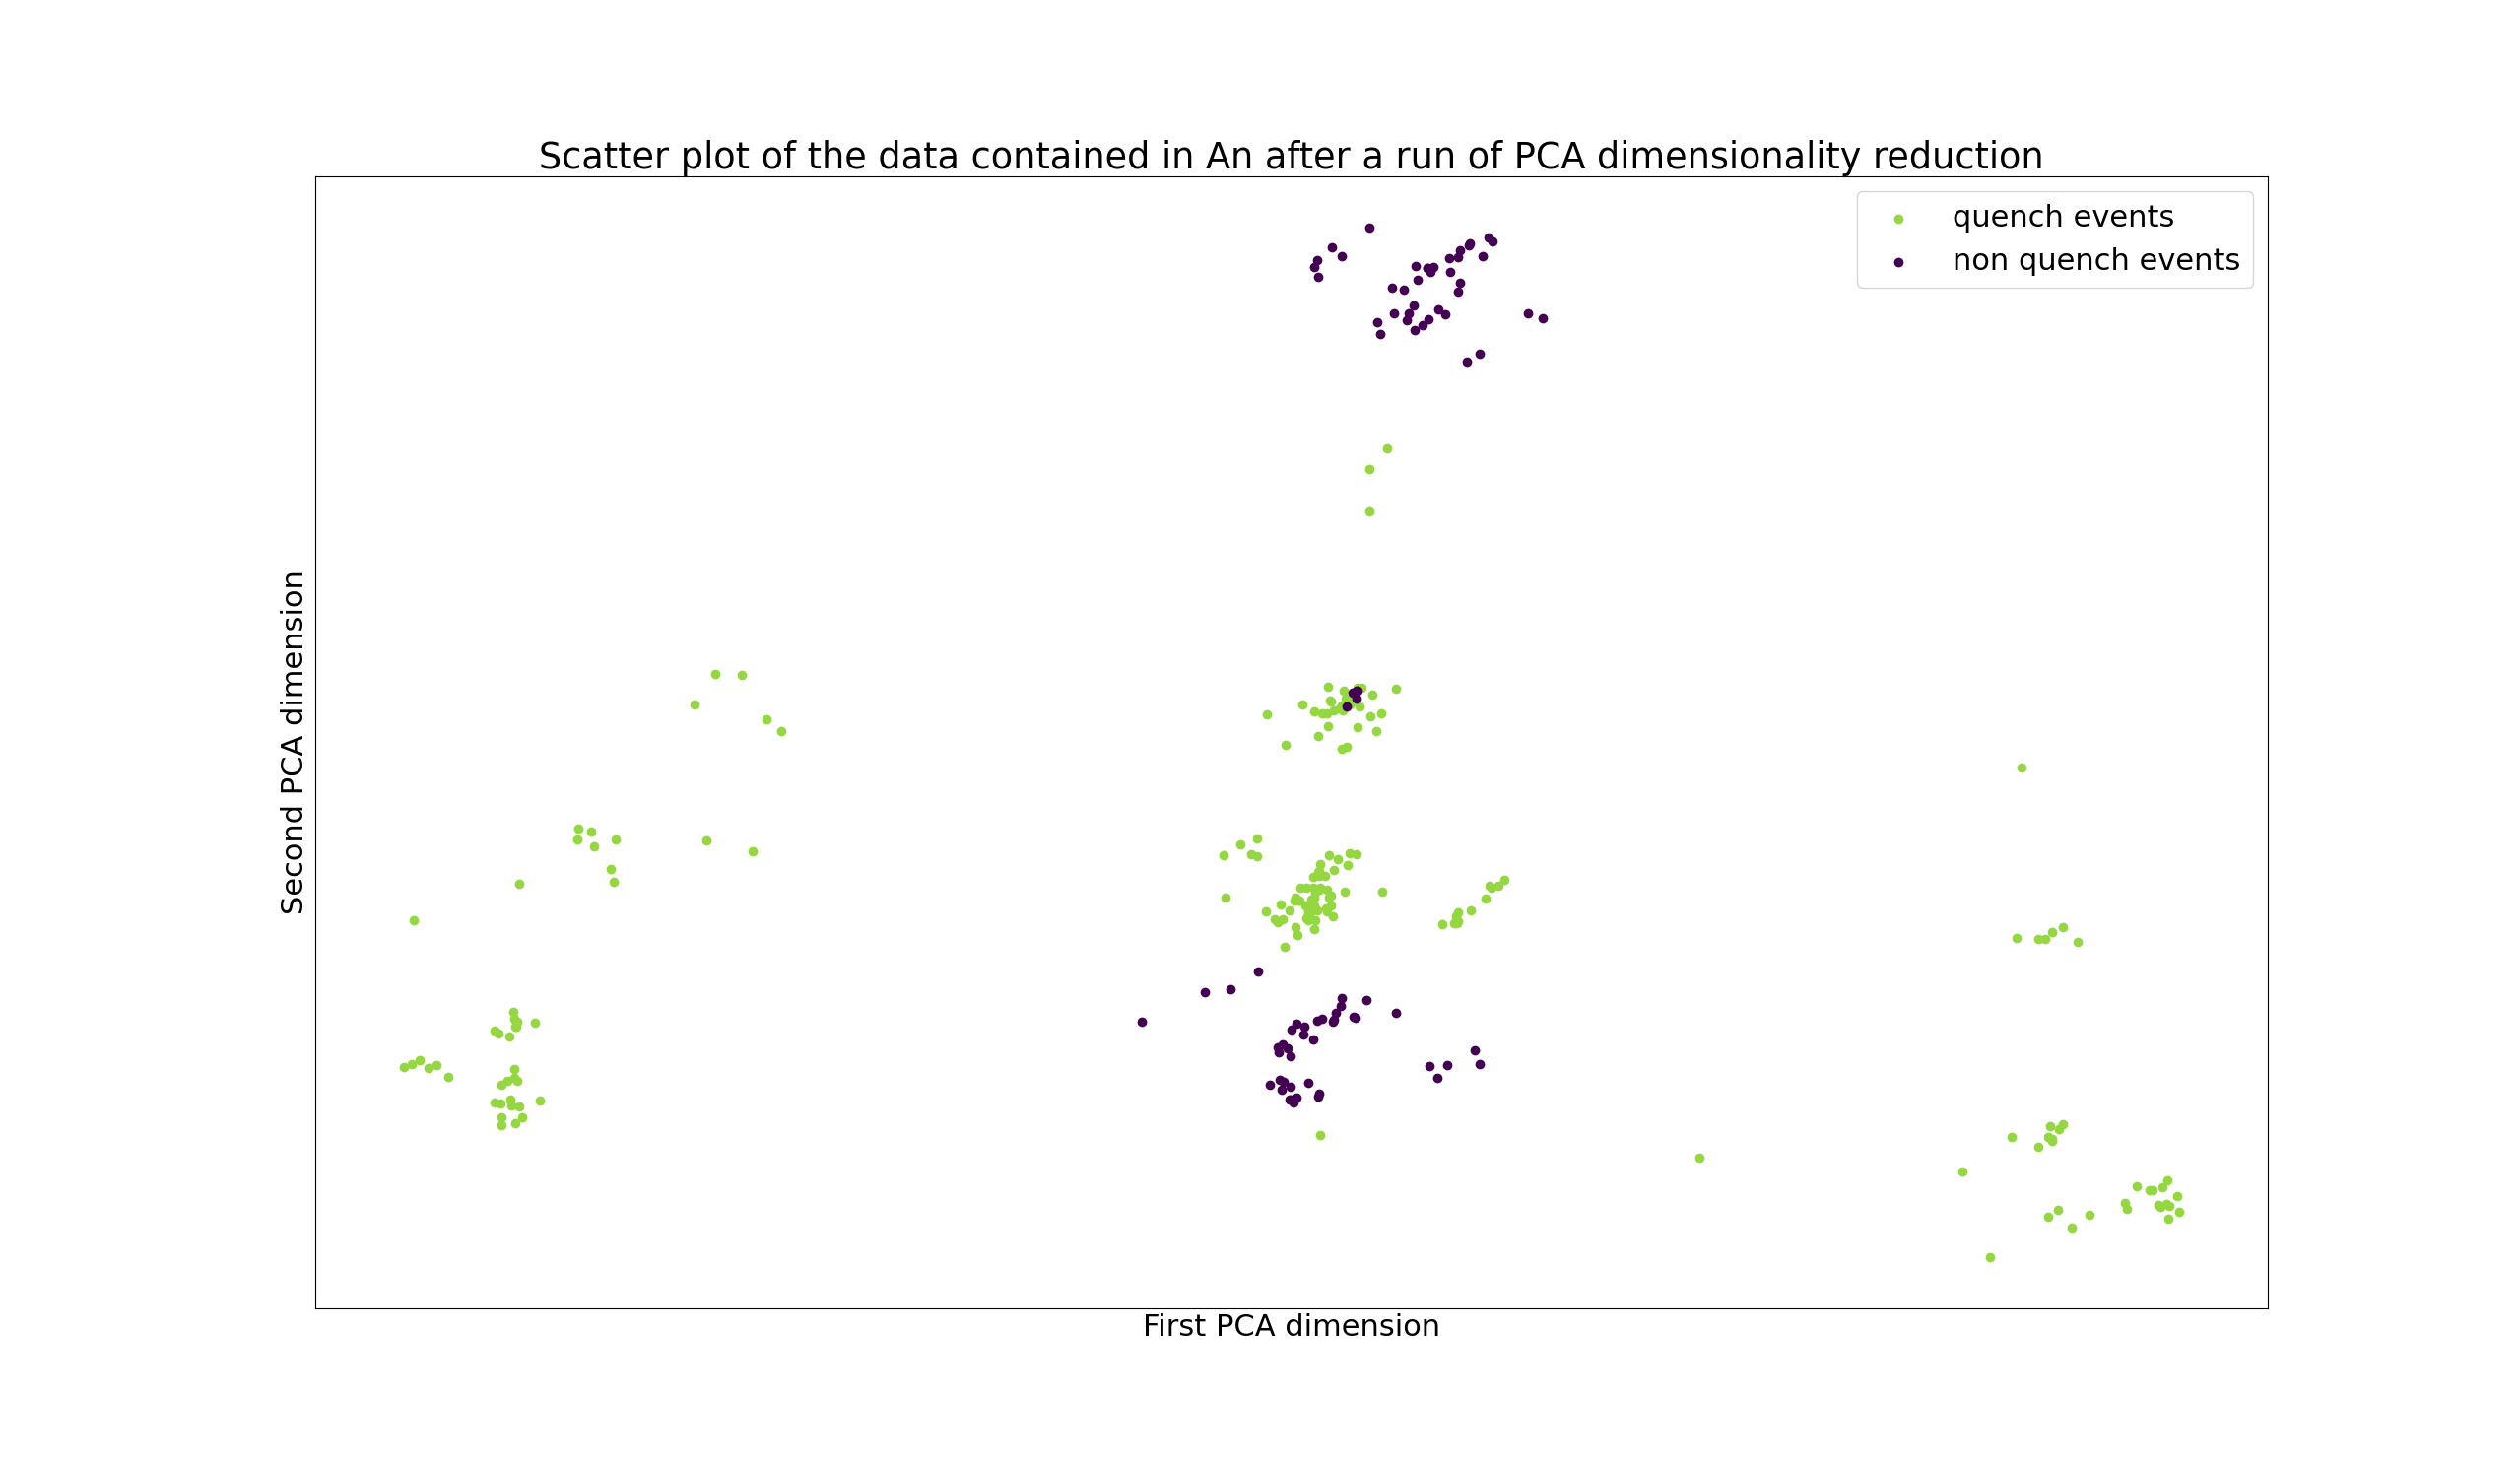
\includegraphics[scale=.23]{img/An_distribution.png}
	\caption{Label correlation for the An table} \label{fig:an-dist}
\end{figure}

As we can see the samples, after dimensionality reduction, are distributed very nicely in a series
of zones, each zone has a very high degree of purity. The very good distribution of the samples must
be the reason why the models built on this table are performing so well.

\subsubsection{Bn table}

\subsubsection{Cnmod table}

\subsubsection{Phi table}

\section{Results}
